\documentclass[12pt]{article}
\usepackage[utf8]{inputenc}
\usepackage{listings} 
\usepackage{minted}
\usepackage{tikz}
\usetikzlibrary{trees}
\usetikzlibrary{shapes,decorations}
\usetikzlibrary {arrows.meta}
\usepackage{graphicx} % Allows you to insert figures
\usepackage{amsmath} % Allows you to do equations
\usepackage{cleveref}
\usepackage{fancyhdr} % Formats the header
%\usepackage{geometry} % Formats the paper size, orientation, and margins
\linespread{1.25} % about 1.5 spacing in Word
\setlength{\parindent}{0pt} % no paragraph indents
\setlength{\parskip}{1em} % paragraphs separated by one line
\usepackage{graphicx} % Required for inserting images


\usepackage[
    left=1in,    % Adjust left margin
    right=1in,   % Adjust right margin
    top=1in,     % Adjust top margin
    bottom=1in   % Adjust bottom margin
]{geometry}
\usepackage{float}
\usepackage{graphicx}  % For including images
\usepackage{tikz}
\usepackage{minted}
\usetikzlibrary{shapes,decorations}
\usetikzlibrary {arrows.meta}

\usetikzlibrary{arrows.meta, positioning}


\title{Figures for ML}
\author{This Document contains all figures used I used in ML}
\date{September 2024}

\begin{document}

\maketitle
\newpage
\section{Semester 1}
\subsection{Advanced Programming}
\subsubsection


\begin{figure}[H]
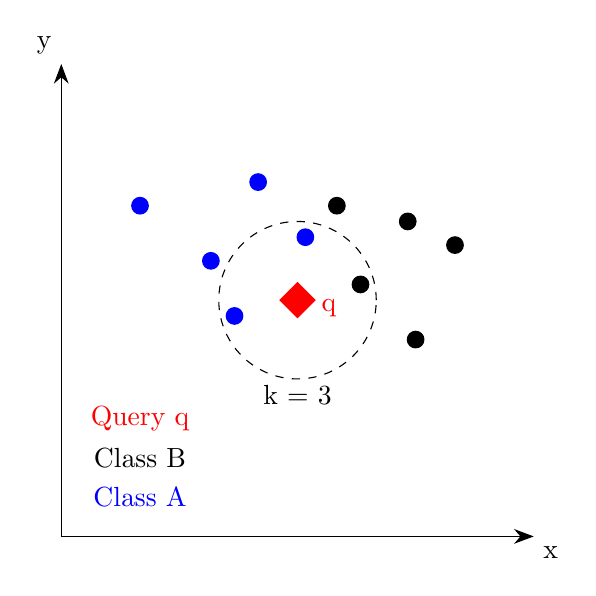
\begin{tikzpicture}
    % Draw x and y axes
    \draw[-{Stealth[length=2.5mm]}] (0,0) -- (6,0) node[anchor=north west] {x};
    \draw[-{Stealth[length=2.5mm]}] (0,0) -- (0,6) node[anchor=south east] {y};

    % Draw class A points (blue)
    \filldraw[blue] (1,4.2) circle (3pt);
    \filldraw[blue] (1.9,3.5) circle (3pt);
    \filldraw[blue] (2.2,2.8) circle (3pt);
    \filldraw[blue] (2.5,4.5) circle (3pt);
    \filldraw[blue] (3.1,3.8) circle (3pt);

    % Draw class B points (green)
    \filldraw (4.5,2.5) circle (3pt);
    \filldraw (3.8,3.2) circle (3pt);
    \filldraw (4.4,4.0) circle (3pt);
    \filldraw (3.5,4.2) circle (3pt);
    \filldraw (5.0,3.7) circle (3pt);
    
    % Draw the query point (red star)
    \node[diamond, fill=red] at (3,3) {};
    \node[red] at (3.4,2.9) {q};
    
    % Draw circles representing K-nearest neighbor areas
    \draw[dashed] (3,3) circle (1);
    %\draw[dashed] (3,3) circle (1.5);

    % Add text for K values
    \node at (3,1.8) {k = 3};
    %\node at (5,2) {k = 7};

    % Add class labels
    \node[blue] at (1,.5) {Class A};
    \node at (1,1) {Class B};
    \node[red] at (1,1.5) {Query q};

\end{tikzpicture}
\qquad
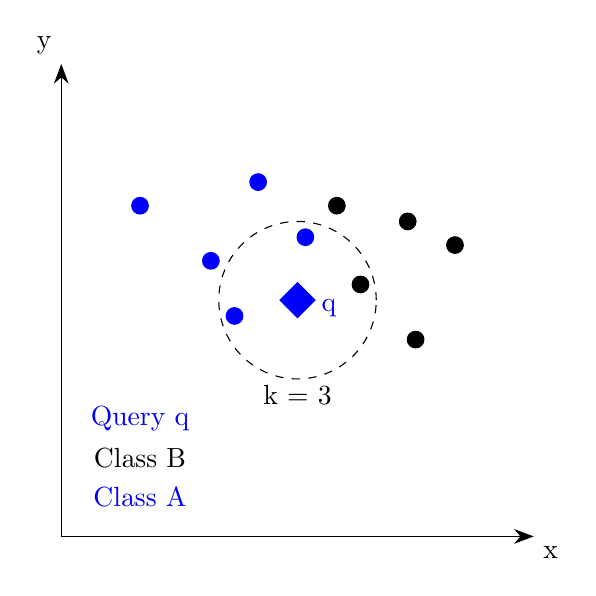
\begin{tikzpicture}
    % Draw x and y axes
    \draw[-{Stealth[length=2.5mm]}] (0,0) -- (6,0) node[anchor=north west] {x};
    \draw[-{Stealth[length=2.5mm]}] (0,0) -- (0,6) node[anchor=south east] {y};


    % Draw class A points (blue)
    \filldraw[blue] (1,4.2) circle (3pt);
    \filldraw[blue] (1.9,3.5) circle (3pt);
    \filldraw[blue] (2.2,2.8) circle (3pt);
    \filldraw[blue] (2.5,4.5) circle (3pt);
    \filldraw[blue] (3.1,3.8) circle (3pt);

    % Draw class B points (green)
    \filldraw (4.5,2.5) circle (3pt);
    \filldraw (3.8,3.2) circle (3pt);
    \filldraw (4.4,4.0) circle (3pt);
    \filldraw (3.5,4.2) circle (3pt);
    \filldraw (5.0,3.7) circle (3pt);
    
    % Draw the query point (red star)
    %\filldraw[blue] (3, 3) circle (4pt);
    \node[diamond, fill=blue] at (3,3) {};
    \node[blue] at (3.4,2.9) {q};
    
    % Draw circles representing K-nearest neighbor areas
    \draw[dashed] (3,3) circle (1);
    %\draw[dashed] (3,3) circle (1.5);

    % Add text for K values
    \node at (3,1.8) {k = 3};
    % \node at (5,2) {k = 7};

    % Add class labels
    \node[blue] at (1,.5) {Class A};
    \node at (1,1) {Class B};
    \node[blue] at (1,1.5) {Query q};

\end{tikzpicture}
\caption{Query point $q$ before and after performing kNN}
\end{figure}
\subsubsection{kD-Trees}

\begin{figure}[H]
\centering
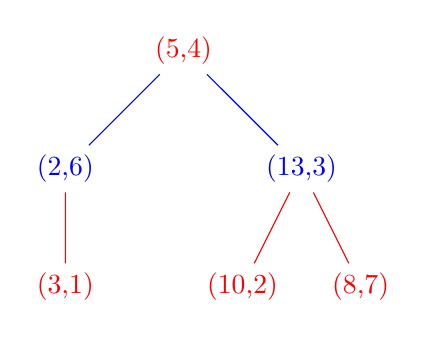
\begin{tikzpicture}[level distance=1.5cm,
  level 1/.style={blue, sibling distance=3cm},
  level 2/.style={red,sibling distance=1.5cm}]
  \node[red] {(5,4)}
    child {node {(2,6)}
      child{node {(3,1)}}
    }
    child {node {(13,3)}
      child {node {(10,2)}}
      child{node {(8,7)}}
    };
    
\end{tikzpicture}
\caption{kD-tree from set $D = [(5,4), (2,6), (13,3), (8,7), (3,1), (10,2)]$} with $k=2$ dimensions\label{fig:kd_tree}
\end{figure}


\subsubsection{kNN with kD-Trees}
\begin{figure}[H]
\centering
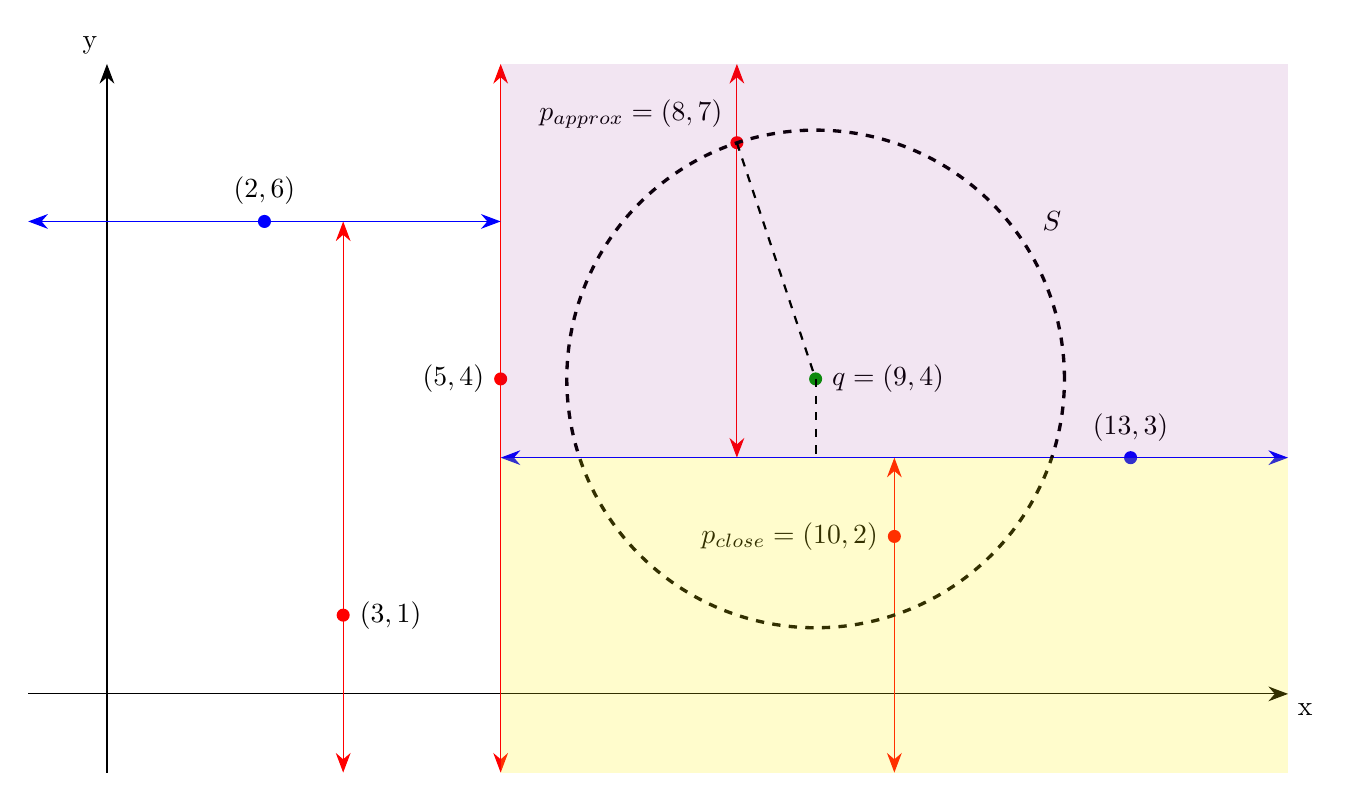
\begin{tikzpicture}[
red_dot/.style={circle, fill=red, scale=0.5},
blue_dot/.style={circle, fill=blue, scale=0.5},
orange_dot/.style={circle, fill=black!40!green, scale=0.5}
]
% Draw x and y axes
    \draw[-{Stealth[length=2.5mm]}] (-1,0) -- (15,0) node[anchor=north west] {x};
    \draw[-{Stealth[length=2.5mm]}] (0,-1) -- (0,8) node[anchor=south east] {y};

% Draw red points from D
    \node[red_dot,label=right:{$(3,1)$}] (n1) at (3,1) {};
    \node[red_dot,label=left:{$(5,4)$}] (n1) at (5,4) {};
    \node[red_dot,label=above left:{$p_{approx}=(8,7)$}] (n1) at (8,7) {};
    \node[red_dot,label=left:{$p_{close}=(10,2)$}] (n1) at (10,2) {};
% Draw blue points from D
    \node[blue_dot,label=above:{$(2,6)$}] (n1) at (2,6) {};
    \node[blue_dot,label=above:{$(13,3)$}] (n1) at (13,3) {};
% Draw q
    \node[orange_dot,label=right:{$q=(9,4)$}] (n1) at (9,4) {};

% Draw vertical lines
    \draw[{Stealth[length=2.5mm]}-{Stealth[length=2.5mm]}, red] (3,-1) -- (3,6){};
    \draw[{Stealth[length=2.5mm]}-{Stealth[length=2.5mm]}, red] (5,-1) -- (5,8){};
    \draw[{Stealth[length=2.5mm]}-{Stealth[length=2.5mm]}, red] (8,3) -- (8,8){};
    \draw[{Stealth[length=2.5mm]}-{Stealth[length=2.5mm]}, red] (10,-1) -- (10,3){};
% Draw horizontal lines
    \draw[{Stealth[length=2.5mm]}-{Stealth[length=2.5mm]}, blue] (-1,6) -- (5,6){};
    \draw[{Stealth[length=2.5mm]}-{Stealth[length=2.5mm]}, blue] (5,3) -- (15,3){};
% Draw S
    \draw[dashed, very thick] (9,4) circle[radius=3.16];
    \node[thick] at (12,6) {$S$};
% Draw bin
    \filldraw[fill=yellow, fill opacity=0.2, draw=none] (5,3) rectangle (15,-1);
    \filldraw[fill=violet, fill opacity=0.1, draw=none] (5,3) rectangle (15,8);
% Draw helper lines
    \draw[dashed, thick] (8,7) -- (9,4);
    \draw[dashed, thick] (9,4) -- (9,3);
\end{tikzpicture}
\caption{From point $(5,4) D$ is split in half and an initial depth first search on the right branch of \cref{fig:kd_tree} is performed and leads to $p_{approx}$. BWB test with sphere $S$ shows that $p_{close}$ is not located in the purple bin and backtracking is performed}\label{fig:M1}
\end{figure}

\subsection{Machine Learning 1}
\subsubsection{Assignment 2}
\subsection{Regression}
\begin{figure}[h]
\centering
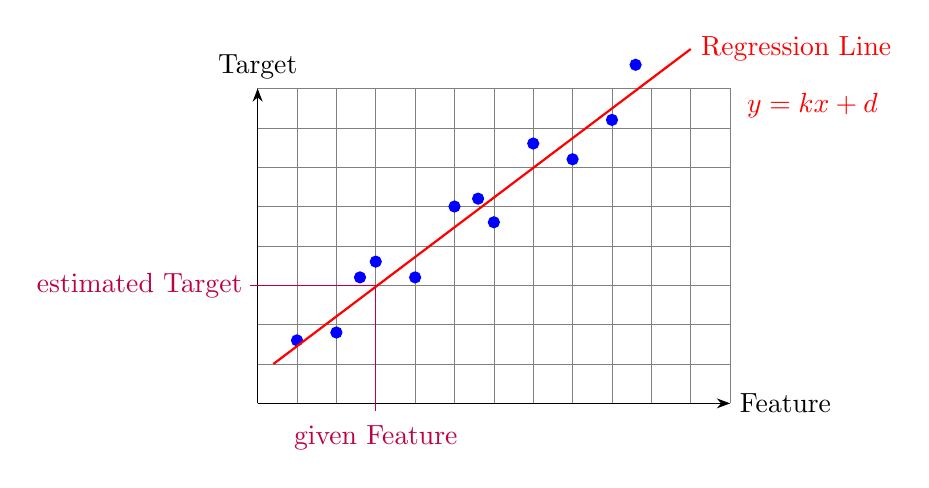
\begin{tikzpicture}[scale=1]

% Draw grid
\draw[step=0.5cm, gray, very thin] (0,0) grid (6,4);
% Draw axes
\draw[-Stealth] (0,0) -- (6,0) node[right] {Feature};
\draw[-Stealth] (0,0) -- (0,4) node[above] {Target};

%Draw example
\draw[purple] (1.5,-0.1) -- (1.5,1.5) node[yshift=-55px] {given Feature};
\draw[purple] (-0.1,1.5) -- (1.5,1.5) node[xshift=-85px] {estimated 
Target};

% Plot data points
\foreach \x/\y in {0.5/0.8, 1/0.9, 1.3/1.6, 1.5/1.8, 2/1.6, 2.5/2.5, 2.8/2.6, 3/2.3, 3.5/3.3, 4/3.1, 4.5/3.6, 4.8/4.3}
{
    \filldraw[blue] (\x,\y) circle (2pt);
}

% Draw regression line
\draw[red, thick] (0.2,0.5) -- (5.5,4.5) node[right] {Regression Line};
\node[above left, red] at (8,3.5) {$y=kx+d$};

\end{tikzpicture}
    \caption{This figure illustrates a regression model applied to a dataset. The blue data points represent observations, such as the relationship between hours studied (Feature) and test scores (Target). The red regression line models this relationship, showing how test scores generally increase with more hours studied. The purple lines demonstrate an example where a specific number of study hours is the input. The expected test score can be estimated by projecting onto the regression line.}
    \label{fig:regression_example}
\end{figure}


\subsection{Classification}

\begin{figure}[H]
\centering
\begin{tikzpicture}[scale=1]

% Draw axes
\draw[-Stealth] (0,0) -- (5,0) node[right] {x};
\draw[-Stealth] (0,0) -- (0,5) node[above] {y};

% Class 1 data points (circles)
\foreach \x/\y in {0.5/3.5, 1/3, 1.5/3.8, 2/4, 2.5/3.5}
{
    \filldraw[blue] (\x,\y) circle (2pt);
}

% Class 2 data points (squares)
\foreach \x/\y in {3/1, 3.5/1.5, 4/1, 4.5/1.8, 3.8/0.5}
{
    % Using nodes
    \node[draw, fill=green!60!black, shape=rectangle, minimum size=4pt, inner sep=0pt] at (\x,\y) {};
}

% Decision boundary
\draw[red, thick] (1,1) -- (4,4);
\node[above left, red] at (6,4) {Decision Boundary};

\end{tikzpicture}
    \caption{This figure depicts a classification problem involving two classes. Blue circles represent one class, such as emails labeled "Spam," and green squares represent another class, like "Not Spam." The red decision boundary separates the two classes based on features. The model uses this boundary to classify new emails as either Spam or Not Spam.}
    \label{fig:regression_example}
\end{figure}

\subsection{Features}

\begin{figure}[H]
\centering
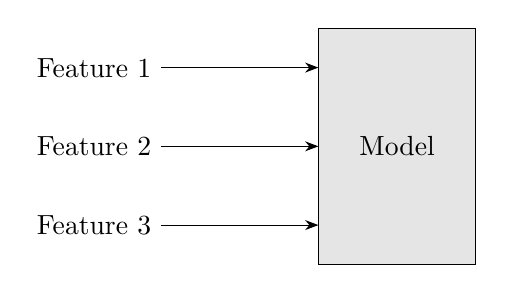
\begin{tikzpicture}

% Draw feature arrows
\node[left] at (0,2) {Feature 1};
\draw[-Stealth] (0,2) -- (2,2);

\node[left] at (0,1) {Feature 2};
\draw[-Stealth] (0,1) -- (2,1);

\node[left] at (0,0) {Feature 3};
\draw[-Stealth] (0,0) -- (2,0);

% Draw model box
\draw[fill=gray!20] (2,-0.5) rectangle (4,2.5) node[midway] {Model};

\end{tikzpicture}
    \caption{This diagram shows three features being input into a machine learning model. For example, in predicting house prices, Feature 1 could be the size of the house in square meters, Feature 2 the number of bedrooms, and Feature 3 the location. These features are fed into the model.}
    \label{fig:regression_example}
\end{figure}

\subsection{Targets}

\begin{figure}[H]
\centering
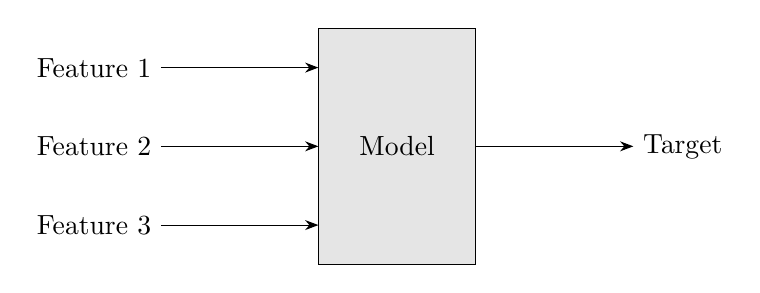
\begin{tikzpicture}

% Draw feature arrows
\node[left] at (0,2) {Feature 1};
\draw[-Stealth] (0,2) -- (2,2);

\node[left] at (0,1) {Feature 2};
\draw[-Stealth] (0,1) -- (2,1);

\node[left] at (0,0) {Feature 3};
\draw[-Stealth] (0,0) -- (2,0);

% Draw model box
\draw[fill=gray!20] (2,-0.5) rectangle (4,2.5) node[midway] {Model};

% Draw target arrow
\draw[-Stealth] (4,1) -- (6,1);
\node[right] at (6,1) {Target};

\end{tikzpicture}
    \caption{Extending figure 3, this figure illustrates the model producing a target output from the input features. After inputting the features, the model outputs a target value, such as the estimated price of the house in Euros.}
    \label{fig:regression_example}
\end{figure}

\subsection{Supervised Machine Learning Workflow}

\begin{figure}[H]
\centering
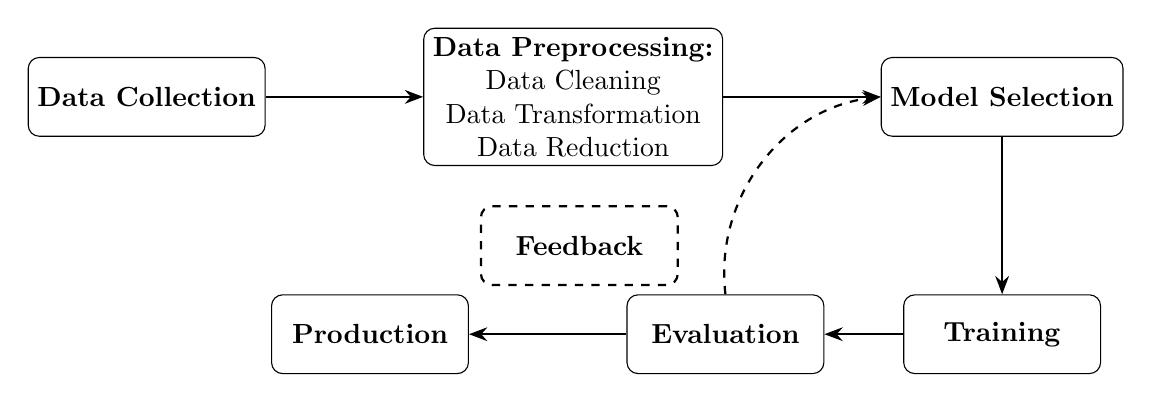
\begin{tikzpicture}[
    node distance=2cm,
    every node/.style={rectangle, draw, rounded corners, align=center, minimum width=2.5cm, minimum height=1cm},
    arrow/.style={-{Stealth}, thick}
    ]

% Nodes
\node (data) {\textbf{Data Collection}};
\node (preprocess) [right=of data] { \textbf{Data Preprocessing:} \\ Data Cleaning \\ Data Transformation \\ Data Reduction};
\node (model) [right=of preprocess] {\textbf{Model Selection}};
\node (training) [below=of model] {\textbf{Training}};
\node (evaluation) [left=of training, xshift=1cm] {\textbf{Evaluation}};
\node (prediction) [left=of evaluation] {\textbf{Production}};

% Arrows
\draw[arrow] (data) -- (preprocess);
\draw[arrow] (preprocess) -- (model);
\draw[arrow] (model) -- (training);
\draw[arrow] (training) -- (evaluation);
\draw[arrow] (evaluation) -- (prediction);

% Optional: Feedback loop from Evaluation to Model Selection
\draw[arrow, dashed] (evaluation.north) to[bend left=45] node[below left, xshift=-30px, yshift=-15px] {\textbf{Feedback}} (model.west);

\end{tikzpicture}
\caption{
This flowchart represents the supervised machine learning workflow. 
The dashed feedback loop indicates that if the evaluation shows low accuracy, the model selection or training process may be revisited to improve performance.
}
    \label{fig:regression_example}
\end{figure}
The steps are:
\begin{enumerate}
    \item \textbf{Data Collection}: Gather images labeled with the objects they contain (e.g., cats and dogs).
    \item \textbf{Data Preprocessing}: Resize images and normalize pixel values.
    \item \textbf{Model Selection}: Choose an appropriate model, like a convolutional neural network (CNN).
    \item \textbf{Training}: Train the CNN using the labeled images.
    \item \textbf{Evaluation}: Assess the model's accuracy in classifying new images.
    \item \textbf{Prediction}: Use the trained model to classify unlabeled images as either cats or dogs.
\end{enumerate}

\newpage

\subsubsection{Assignment 3}
\subsection{Train-Test Split}

\begin{figure}[h]
\centering
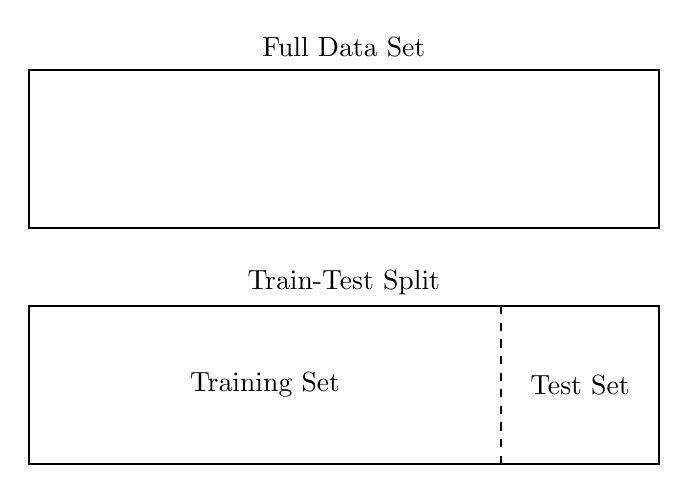
\begin{tikzpicture}[scale=1]

\node at (4, 5.3) {Full Data Set};
\draw[thick] (0,3) rectangle (8,5);

% Split train and test rectangle
\draw[thick] (0,0) rectangle (8,2);
\node at (4, 2.3) {Train-Test Split};

% Dashed line for splitting train and test
\draw[dashed, thick] (6,0) -- (6,2);
\node at (3, 1) {Training Set };
\node at (7, 1) {Test Set };

\end{tikzpicture}
    \caption{The Train-Test split is applied on data to split the test in training data and test data that is unseen to the model to validate it. A typical split ratio is $80\%$ training data and $20\%$ test data. }
\end{figure}
It is important to shuffle the data before processing because of many reasons. Some of the most imortant are: 
\begin{itemize}
    \item \textbf{Break order based patterns:} shuffling prevents models from learning unintended dependencies on data order (e.g. is often gathered in certain groups).
    \item \textbf{Reduce bias and overfitting:} ensure diverse data represantation in every batch of training data.
    \item \textbf{Generalization and effectiveness:} to ensure the model is able to learn meaningful patterns and perform well on unseen data .
\end{itemize}
\subsection{Mean Absolute Error}

The formula for Mean Absolute Error (MAE) is given by:

\[MAE = \frac{1}{n} \sum_{i=1}^{n} | y_i - \hat{y}_i |\]
Where:
\begin{itemize}
    \item \(n\) is the total number of observations.
    \item \(y_i\) is the actual value for the \(i\)-th observation.
    \item \(\hat{y}_i\) is the predicted value for the \(i\)-th observation.
    \item \( | y_i - \hat{y}_i | \) is the absolute difference between the actual and predicted values.
\end{itemize}

MAE measures the average magnitude of errors between the predicted values and actual values, treating all errors equally. For example if a model wants to predict the location of an object in an image. The actual coordinates of the top-left corner are \((50, 100)\), while the predicted coordinates are \((55, 90)\).

To calculate the Mean Absolute Error (MAE):

\begin{itemize}
    \item \textbf{Actual Coordinates}: \((50, 100)\)
    \item \textbf{Predicted Coordinates}: \((55, 90)\)
    \item Absolute error for the x-coordinate: \( |50 - 55| = 5 \)
    \item Absolute error for the y-coordinate: \( |100 - 90| = 10 \)
\end{itemize}

The MAE for this prediction is:
\[MAE = \frac{5 + 10}{2} = 7.5\]

This means the average error in object location prediction is 7.5 pixels.
\\
While MAE treats all errors equally by calculating the average of absolute differences and therefore makes it less sensitive to outliers, the Root Mean Squared Error (RMSE) squares the errors before averaging, giving more weight to larger errors. This means RMSE is more sensitive to outliers, as large deviations are amplified.


\subsection{Accuracy}
\begin{figure}[h]
\centering
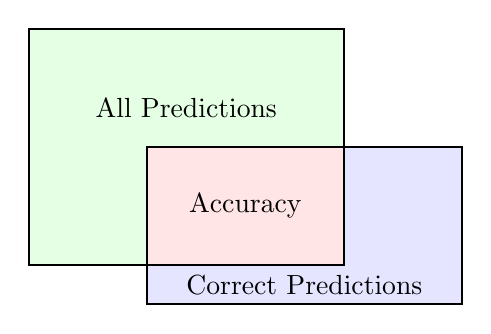
\begin{tikzpicture}[scale=1]
% Draw two boxes for predicted and actual labels
\draw[thick,fill=green!10] (0, 0) rectangle (4, 3){};
\draw[thick, fill=blue!10] (1.5, -0.5) rectangle (5.5, 1.5) node[midway]{}; 
\node at (2, 2) {All Predictions};
\node at (3.5, -0.25) {Correct Predictions};
% Intersection (correct predictions)
%\draw[fill=green!30, thick] (0.5, 0.5) rectangle (2.5, 1.5);
%\node at (1.5, 1) {Correct};

\draw[thick, fill=red!10] (1.5, 0) rectangle (4, 1.5) node[midway] {Accuracy};

\end{tikzpicture}
    \caption{This diagram shows the overlap between all predictions (green) and correct predictions (blue), with the overlapping area corresponding to the accuracy. The bigger the overlap is, the higher the model's accuracy. Very sensitive to class imbalance (more positives than negatives).}
\end{figure}

\[ Accuracy = \frac{Correct\,Predictions}{All\,Predictions} = \frac{TP+TN}{TP+TN+FP+FN} \]
\subsection{Confusion Matrix (Snippet)}
\begin{figure}[H]
\centering
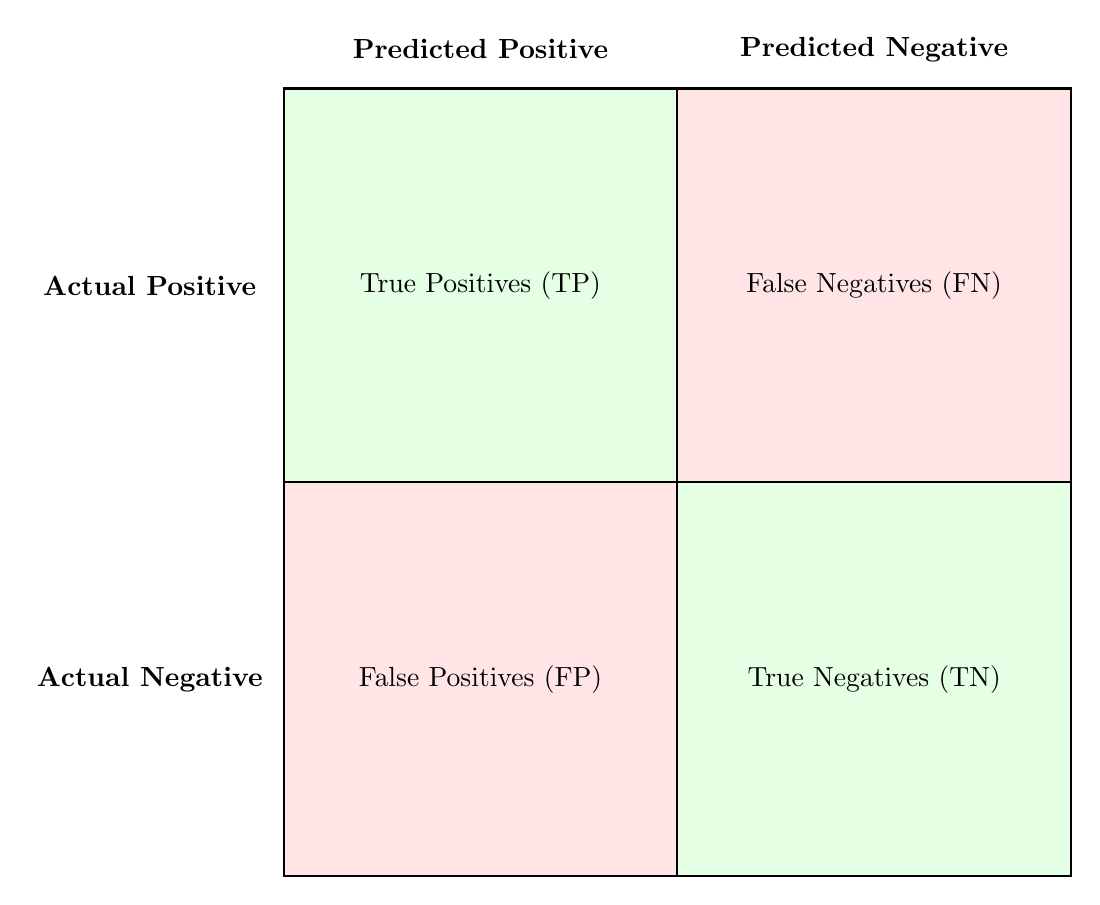
\begin{tikzpicture}[scale=1]
% Confusion matrix
\draw[thick] (0,0) rectangle (10, 10);  % Outer box for confusion matrix
\draw[dashed, thick] (5, 0) -- (5, 10); % Vertical dashed line for split
\draw[dashed, thick] (0, 5) -- (10, 5); % Horizontal dashed line for split

% Labels for axes
\node at (-1.7, 7.5) {\textbf{Actual Positive}};
\node at (-1.7, 2.5) {\textbf{Actual Negative}};
\node at (2.5, 10.5) {\textbf{Predicted Positive}};
\node at (7.5, 10.5) {\textbf{Predicted Negative}};

% Labels inside the confusion matrix
\draw[thick,fill=green!10] (0, 5) rectangle (5, 10){};
\node at (2.5, 7.5) {True Positives (TP)};  % Top-left quadrant

\draw[thick,fill=red!10] (5, 5) rectangle (10, 10){};
\node at (7.5, 7.5) {False Negatives (FN)}; % Top-right quadrant

\draw[thick,fill=red!10] (0, 0) rectangle (5, 5){};
\node at (2.5, 2.5) {False Positives (FP)}; % Bottom-left quadrant

\draw[thick,fill=green!10] (5, 0) rectangle (10, 5){};
\node at (7.5, 2.5) {True Negatives (TN)};  % Bottom-right quadrant


% Highlight True Positives
%\draw[fill=green!30, thick] (0, 1.5) rectangle (1.5, 3);

\end{tikzpicture}
    \caption{Confusion Matrix is a table to evaluate the performance of a model by comparing predicted labels with actual labels. The rows are actual and the columns are predicted labels}
\end{figure}
    The steps are:
\begin{enumerate}
    \item \textbf{True Positives}: Correctly predicted positive cases (e.g., cars that are labeled as cars).
\item \textbf{False Positives}: Incorrectly predicted positive cases (e.g., buses predicted as cars).
\item \textbf{True Negatives}: Correctly predicted negative cases (e.g., buses predicted as not cars).
\item \textbf{False Negatives}: Incorrectly predicted negative cases (e.g., cars predicted as not cars).
\end{enumerate}

\subsubsection{True Positive Rate (Sensitivity)}
The True-Positive Rate (TPR) measures the correctly identified labels. TPR is crucial when missing positive cases is costly (e.g. stop sign detection for self driving car). Not sensitive to True Negatives. It is defined by:
\[ TPR = \frac{TP}{TP+FN}\]

\subsubsection{True Negative Rate (Specicivity)}
The True-Negative Rate measures the proportion of actual negatives correctly identified. A high TNR is crucial when avoiding false positives is crucial (e.g. marking credit card transactions as non fraud). It is defined by: 
\[ TNR = \frac{TN}{TN+FP}\]

\subsubsection{Assignment 4}
Explain “hyper parameters“ and “K nearest neighbours“ in your own words.
\subsection{Hyperparameters}
\begin{figure} [h]
		\begin{center}  
			\subfigure 
			{ 
				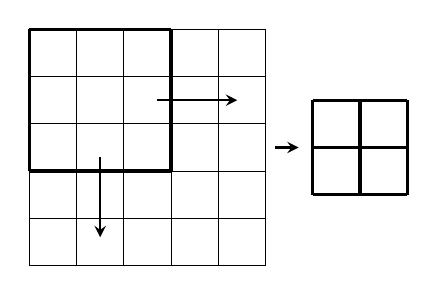
\begin{tikzpicture}[scale=.6]
					\draw [thin](0,0) grid (5,5);
					\draw[very thick] (0,5) to(3,5);
					\draw[very thick] (0,2) to(3,2);
					\draw[very thick] (0,5) to(0,2);
					\draw[very thick] (3,2) to(3,5);
					\draw[->,>=stealth,thick](2.7,3.5) to (4.4,3.5);
					\draw[->,>=stealth,thick](1.5,2.3) to (1.5,0.6);
					\draw[->,>=stealth,thick](5.2,2.5) to (5.7,2.5);
					\draw[very thick] (6,1.5) to(6,3.5);
					\draw[very thick] (8,1.5) to(8,3.5);
					\draw[very thick] (6,1.5) to(8,1.5);
					\draw[very thick] (6,3.5) to(8,3.5);
					\draw[very thick] (6,2.5) to(8,2.5);
					\draw[very thick] (7,1.5) to(7,3.5);
				\end{tikzpicture}
			}
		\hspace{1cm}
			\subfigure 
			{ 
				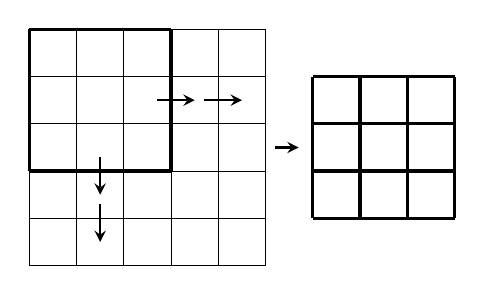
\begin{tikzpicture}[scale=.6]
					\draw [thin](0,0) grid (5,5);
					\draw[very thick] (0,5) to(3,5);
					\draw[very thick] (0,2) to(3,2);
					\draw[very thick] (0,5) to(0,2);
					\draw[very thick] (3,2) to(3,5);
					\draw[->,>=stealth,thick](2.7,3.5) to (3.5,3.5);
					\draw[->,>=stealth,thick](3.7,3.5) to (4.5,3.5);
					\draw[->,>=stealth,thick](1.5,2.3) to (1.5,1.5);
					\draw[->,>=stealth,thick](1.5,1.3) to (1.5,0.5);
					\draw[->,>=stealth,thick](5.2,2.5) to (5.7,2.5);
					\draw[very thick] (6,4) to(6,1);
					\draw[very thick] (7,4) to(7,1);
					\draw[very thick] (8,4) to(8,1);
					\draw[very thick] (9,4) to(9,1);
					\draw[very thick] (9,4) to(6,4);
					\draw[very thick] (9,3) to(6,3);
					\draw[very thick] (9,2) to(6,2);
					\draw[very thick] (9,1) to(6,1);
					
				\end{tikzpicture}
			}
			\caption{Example of stride}
		\end{center}
	\end{figure}
 Hyper parameters are external configuration variables to manage machine learning training. They are determined through tests and are not obtained from the actual data. They determine how a model learns and are therefore critical for fine-tuning. Examples include:
 \begin{itemize}
     \item Stride: Step size of filter
     \item Filter Size: Size of sliding window
     \item Learning rate: Step size towards minimum of loss function in one iteration
     \item Batch size: Number of training samples used in one iteration
 \end{itemize}
        
\newpage
\subsection{K-Nearest-Neighbours}

\begin{figure}[H]
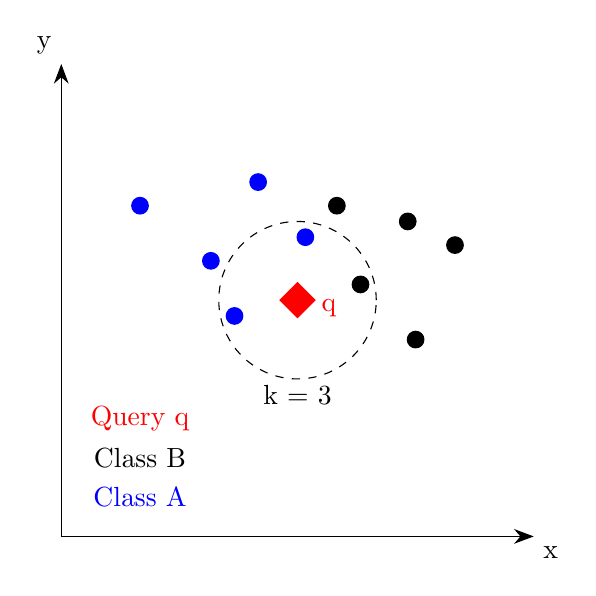
\begin{tikzpicture}
    % Draw x and y axes
    \draw[-{Stealth[length=2.5mm]}] (0,0) -- (6,0) node[anchor=north west] {x};
    \draw[-{Stealth[length=2.5mm]}] (0,0) -- (0,6) node[anchor=south east] {y};

    % Draw class A points (blue)
    \filldraw[blue] (1,4.2) circle (3pt);
    \filldraw[blue] (1.9,3.5) circle (3pt);
    \filldraw[blue] (2.2,2.8) circle (3pt);
    \filldraw[blue] (2.5,4.5) circle (3pt);
    \filldraw[blue] (3.1,3.8) circle (3pt);

    % Draw class B points (green)
    \filldraw (4.5,2.5) circle (3pt);
    \filldraw (3.8,3.2) circle (3pt);
    \filldraw (4.4,4.0) circle (3pt);
    \filldraw (3.5,4.2) circle (3pt);
    \filldraw (5.0,3.7) circle (3pt);
    
    % Draw the query point (red star)
    \node[diamond, fill=red] at (3,3) {};
    \node[red] at (3.4,2.9) {q};
    
    % Draw circles representing K-nearest neighbor areas
    \draw[dashed] (3,3) circle (1);
    %\draw[dashed] (3,3) circle (1.5);

    % Add text for K values
    \node at (3,1.8) {k = 3};
    %\node at (5,2) {k = 7};

    % Add class labels
    \node[blue] at (1,.5) {Class A};
    \node at (1,1) {Class B};
    \node[red] at (1,1.5) {Query q};

\end{tikzpicture}
\qquad
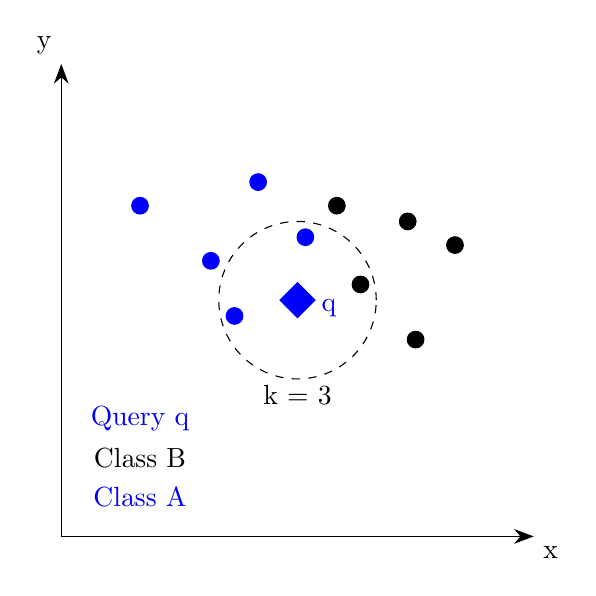
\begin{tikzpicture}
    % Draw x and y axes
    \draw[-{Stealth[length=2.5mm]}] (0,0) -- (6,0) node[anchor=north west] {x};
    \draw[-{Stealth[length=2.5mm]}] (0,0) -- (0,6) node[anchor=south east] {y};


    % Draw class A points (blue)
    \filldraw[blue] (1,4.2) circle (3pt);
    \filldraw[blue] (1.9,3.5) circle (3pt);
    \filldraw[blue] (2.2,2.8) circle (3pt);
    \filldraw[blue] (2.5,4.5) circle (3pt);
    \filldraw[blue] (3.1,3.8) circle (3pt);

    % Draw class B points (green)
    \filldraw (4.5,2.5) circle (3pt);
    \filldraw (3.8,3.2) circle (3pt);
    \filldraw (4.4,4.0) circle (3pt);
    \filldraw (3.5,4.2) circle (3pt);
    \filldraw (5.0,3.7) circle (3pt);
    
    % Draw the query point (red star)
    %\filldraw[blue] (3, 3) circle (4pt);
    \node[diamond, fill=blue] at (3,3) {};
    \node[blue] at (3.4,2.9) {q};
    
    % Draw circles representing K-nearest neighbor areas
    \draw[dashed] (3,3) circle (1);
    %\draw[dashed] (3,3) circle (1.5);

    % Add text for K values
    \node at (3,1.8) {k = 3};
    % \node at (5,2) {k = 7};

    % Add class labels
    \node[blue] at (1,.5) {Class A};
    \node at (1,1) {Class B};
    \node[blue] at (1,1.5) {Query q};

\end{tikzpicture}
\caption{Query point $q$ before and after performing kNN}
\end{figure}
K-nearest-neighbours (KNN) is a machine learning algorithm. it classifies points based on majority vote of it's $k$ nearest neighbours. K and the distance metric are hyper-parameters the output depends heavily on it. KNN works works by calculating the distance from each point in the dataset to the query point (lazy learning). \\
\begin{itemize}
    \item k: The value of $k$ significantly affects performance. A small K is sensitive to noise, while a large K might over-generalize.
    \item Distance Metric: is used to calculate how close two points are (e.g Manhattan, Euclidian)
\end{itemize}

\newpage 
\subsubsection{Assignment 5}
\subsection{Missing Data}


\begin{figure}[h]
\centering
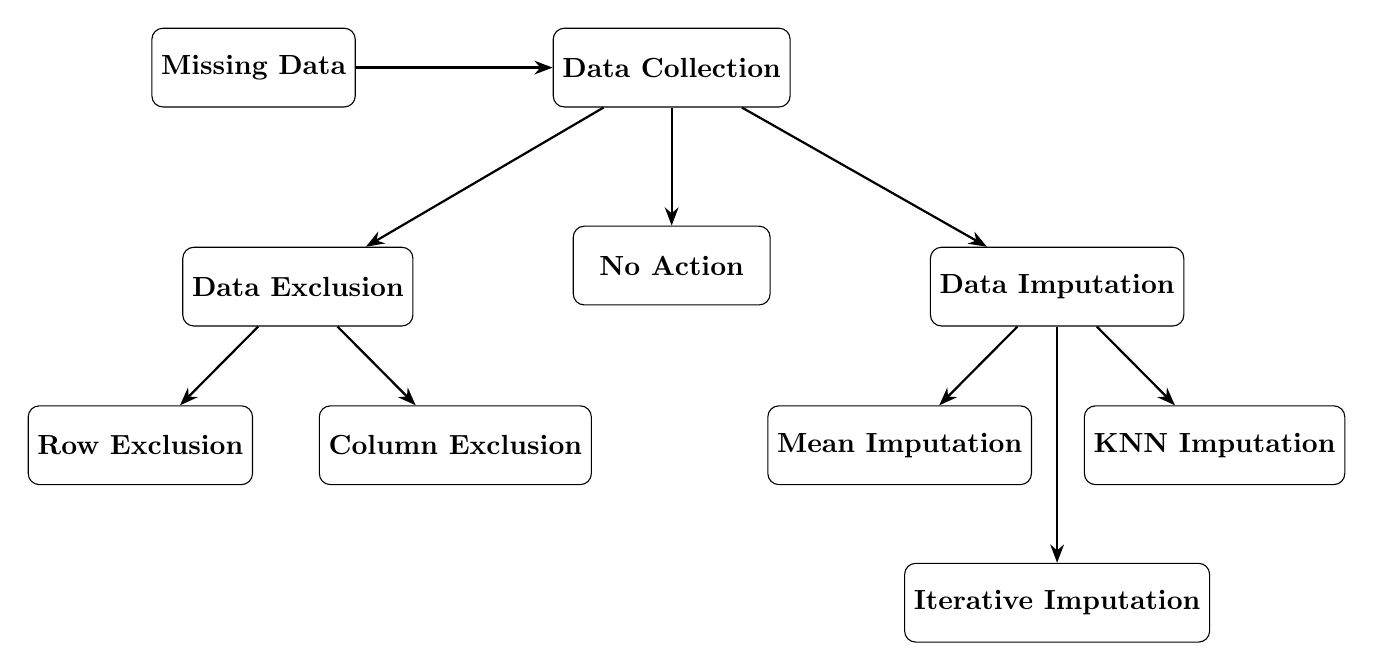
\begin{tikzpicture}[
    node distance=2.5cm,
    every node/.style={rectangle, draw, rounded corners, align=center, minimum width=2.5cm, minimum height=1cm},
    arrow/.style={-{Stealth}, thick}
    ]

% Nodes
\node (start) {\textbf{Missing Data}};

\node (collect) [right=of start] {\textbf{Data Collection}};
\node (nothing) [below=of collect, yshift=1cm] {\textbf{No Action}};
\node (exclude) [below left=of collect] {\textbf{Data Exclusion}};
\node (impute) [below right=of collect] {\textbf{Data Imputation}};

% Sub nodes for Exclusion
\node (row_excl) [below=1cm of exclude, xshift=-2cm] {\textbf{Row Exclusion}};
\node (col_excl) [below=1cm of exclude, xshift=2cm] {\textbf{Column Exclusion}};

% Sub nodes for Imputation
\node (mean_imp) [below=1cm of impute, xshift=-2cm, yshift=0cm] {\textbf{Mean Imputation}};
\node (knn_imp) [below=1cm of impute, xshift=2cm] {\textbf{KNN Imputation}};
\node (iter_imp) [below=3cm of impute] {\textbf{Iterative Imputation}};

% Arrows
\draw[arrow] (start) -- (collect);
\draw[arrow] (collect) -- (nothing);
\draw[arrow] (collect) -- (exclude);
\draw[arrow] (collect) -- (impute);
\draw[arrow] (exclude) -- (row_excl);
\draw[arrow] (exclude) -- (col_excl);
\draw[arrow] (impute) -- (mean_imp);
\draw[arrow] (impute) -- (knn_imp);
\draw[arrow] (impute) -- (iter_imp);

\end{tikzpicture}
\caption{Methods for Handling Missing Data}
\end{figure}
When dealing with missing data there are several strategies for different scenarios. They can broadly be categorized into collection, exclusion, imputation:
\begin{itemize}
    \item\textbf{Data Collection}: best way to adress missing data is to collect it through further data gathering
    \item\textbf{Data Exclusion}: if collection more data is not feasable either \textbf{rows} or \textbf{cols} can be dropped. But this can introduce bias.
    \item \textbf{Data Imputation}: missing values can be filled by:
    \begin{itemize}
        \item \textbf{Mean Imputation}: fill with mean value of the column.
        \item \textbf{Iterative Imputation}: use a regression model to to predict the missing values.
        \item \textbf{KNN Imputation}: use knn algorithm to predict missing values based on similar data points.
    \end{itemize}
    \item \textbf{No Action}: in some case algorithms can handle missing values.
\end{itemize}
\end{document}
